\chapter{Autonomous Navigation}

\textbf{Author: Lukas Leskovar} 
Autonomy or the capability of a robot to perform certain tasks without human supervision or intervention is a central topic in any robotic applications.
While stationary systems performing repetitive tasks can be automated relatively effortlessly, mobile robots introduce many challenges that need to be overcome in order to achieve autonomy.
This chapter deals with the classification and explanation of such robots to illustrate the applicability of Autumn as a autonomous navigation system.

\section{Autonomous Navigation}
To navigate a robot trough its environment autonomously it is necessary to develop an algorithm that employs the robot to move without any external controls. Regardless of how this algorithm is implemented any autonomous mobile vehicle consists of two fundamental abilities. The ability to perceive its surroundings using one or many sensors and to relocate itself using actuators. 

\subsection{Reactive Approach}

\begin{figure}
	\centering
	\includegraphics[width=0.9\linewidth]{img/reactive}
	\caption{
		A reactive control cycle matching sensor inputs directly to actions.
	}
	\label{fig:reactiveApproach}
\end{figure}

One way to autonomously control a robot is to define simple behavioural rules that directly act upon sensory input without needing a sophisticated model of its environment. 
This approach can be associated with bionic robotics as its concepts are inspired by relatively simple life forms performing intelligent behaviour without having a brain. 
A control cycle following this approach can be seen in Fig. \ref{fig:reactiveApproach}

These behaviours match sensory input to movement and can be categorized into three levels of complexity:
\begin{itemize}
	\item Reflexes - pre programmed direct connections between stimuli and actions
	\item Reactions - learned behaviours that execute without the need of complex logic 
	\item Consciousness - sequences of reactive behaviours ruled by a logic architecture
\end{itemize}

Within a reactive system different behaviours are stacked without any knowledge of one another. This allows for layers to build upon functionality implemented by lower layers while maintaining decoupling of modules thus promoting task dissection and facilitate independent testing \footcite{faigl2017controlParadigms}.
%Robotic Paradigms and Control Architectures Jan Faigl


\subsection{Hierarchical Approach}
Contrary to reactive systems robots representing the hierarchical approach require a much more complex implementation as world modelling and sophisticated reasoning is needed. 
Any such system, as seen in Fig. \ref{fig:hierarchicalApproach}, can be divided into three components that are executed sequentially:
\begin{itemize}
	\item Sense - the robot perceives its environment and creates an abstracted model of it (e.g. create a occupancy grid using a LiDAR sensor)
	\item Plan - using a model of the environment (e.g. find the shortest path to a given waypoint)
	\item Act - transform the plan into motion by controlling the robots manipulators
\end{itemize}

While this approach can introduce many difficulties concerning real-world representation or computational complexity this approach facilitates development of intelligent semi- or fully-autonomous vehicles \footcite{faigl2017controlParadigms} \footcite{burgard2020controlParadigms}.

\begin{figure}
	\centering
	\includegraphics[width=0.9\linewidth]{img/hierarchical}
	\caption{
		A hierarchical control system executing the sense, plan, act cycle sequentially.
	}
	\label{fig:hierarchicalApproach}
\end{figure}

\subsection{Hybrid Approach}

\begin{figure}
	\centering
	\includegraphics[width=0.9\linewidth]{img/hybrid}
	\caption{
		A hybrid control system with a planning module supervising a reactive structure. 
	}
	\label{fig:hybridApproach}
\end{figure}


One way to combine the reactive paradigms simplicity with the intricate prevision of tasks as seen in hierarchical systems can be implemented using a hybrid approach, which is depicted in Fig. \ref{fig:hybridApproach}. 
This concept uses deliberate planning algorithms to determine which reactive behaviour should be executed using a global world model, all while monitoring the success of each behaviour to determine if its beneficial to achieve a set goal (e.g find out if the robot moves to a waypoint or is stuck) \footcite{faigl2017controlParadigms}.
%Robotic Paradigms and Control Architectures Jan Faigl

\section{Difficulties}
%While in theory many approaches are applicable to a robot achieving autonomy can still be a challenging task due to many irregularities in its environment. 
While in theory many approaches are applicable to a robot, achieving autonomy can still be a challenging task. Difficulties may arise due to the following reasons:
\begin{itemize}
	\item Sensing Inaccuracy - Sensors are inherently inaccurate, which can greatly affect how the robot observes its environment and the thereby resulting model. Means of improving sensory measurements usually employ data or sensor fusion methods \footcite[Page 585]{siciliano2008springer}.
	\item Dynamic Environments - Its relatively easy for a robot to locate itself within a static environment as its pose is the only variable. However many difficulties may arise when irregularities such as people, movable objects, doors, etc. are introduced. These dynamic properties may be treated as noise and thus be filtered \footcite[Pages 159 - 162]{thrun2002probabilisticRobotics}.
	\item Predictability of Motion - The actuators robots are equipped with do not exactly perform motion as in any predicted model. This may be due to inaccuracies in actuator fabrication, uneven terrain or changing wind conditions. To counteract such tendencies motion control paradigms can be applied \footcite[Page 133]{siciliano2008springer}
\end{itemize}

\section{Autonomous Navigation in Autumn}\label{autumnControlLoop}
The preceding sections described in great detail how a mobile robot can achieve autonomous navigation and which difficulties may hinder development of such system. Autumn and its use-case does not differ from any such system which rendered the question how autonomy is achieved to be central concern during the development phase. 
In order to achieve the best possible product with the available hardware, a semi-autonomous approach was chosen, whose control structure is described in Fig. \ref{fig:autumnControlLoop}.
The individual interchangeable components the system consists of are described in further chapters.

\begin{figure}
	\centering
	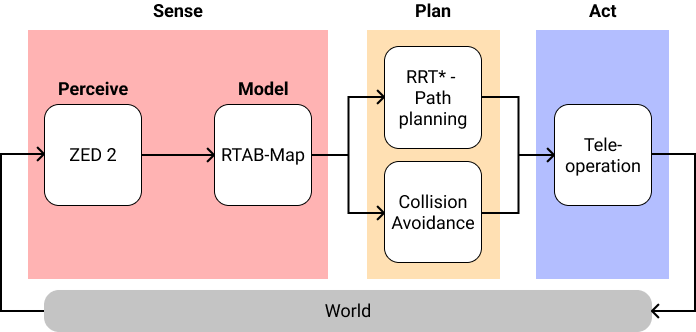
\includegraphics[width=0.9\linewidth]{img/AutumnControlCycle}
	\caption{
		This diagram depicts how a hierarchical control system is implemented within Autumn. Using the data provided by a Stereolabs ZED 2 stereo-camera, a abstracted model of the drones environment is created. This model is utilized by path planning and collision avoidance algorithms to propose the best possible path to a given waypoint. A drone pilot can navigate the quadrocopter through a hazardous environment given this path. 
	}
	\label{fig:autumnControlLoop}
\end{figure}

%Controll Cylcle (Sense, Perceive, Plan, Act)

\filbreak